\documentclass[border=4pt]{standalone}

\usepackage[T1]{fontenc}
\usepackage[utf8]{inputenc}
\usepackage{amsmath}
\usepackage{xcolor}
\usepackage{tikz}
\usetikzlibrary{arrows.meta}

\begin{document}

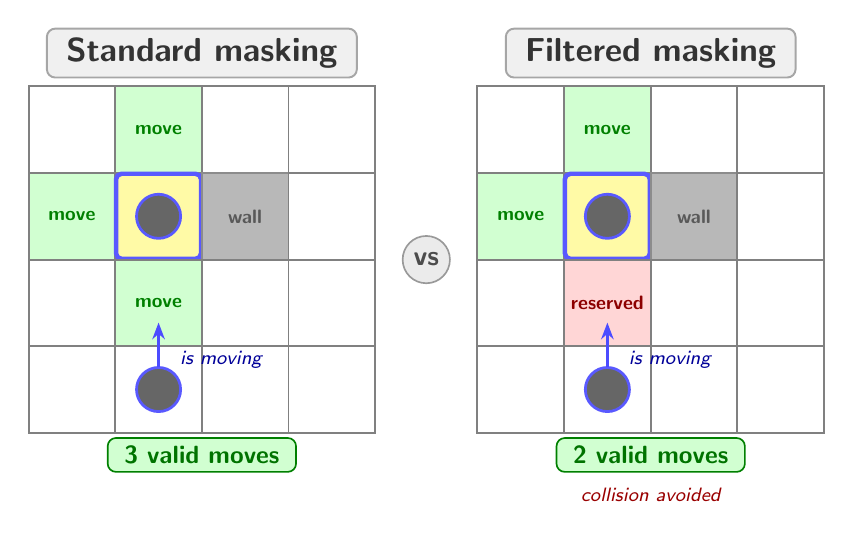
\begin{tikzpicture}[
    cell/.style={minimum size=1.1cm, draw=black!50, line width=0.7pt, inner sep=0pt},
    valid/.style={cell, fill=green!18},
    wall/.style={cell, fill=black!28, draw=black!45},
    reserved/.style={cell, fill=red!16},
    selected/.style={cell, fill=yellow!35},
    empty/.style={cell, fill=white},
    % ── soft pill headings ──
    hpill/.style={fill=black!6, draw=black!35, line width=0.7pt, text=black!80, rounded corners=3pt,
                  anchor=south, inner xsep=7pt, inner ysep=3.5pt, font=\large\bfseries\sffamily},
    % ── result badges ──
    goodpill/.style={fill=green!18, draw=green!50!black, line width=0.6pt, text=green!45!black,
                     rounded corners=3pt, anchor=north, inner xsep=6pt, inner ysep=3pt, font=\small\bfseries\sffamily},
    celllabel/.style={font=\scriptsize\bfseries\sffamily},
    movelabel/.style={font=\scriptsize\itshape\sffamily, text=blue!60!black, anchor=south west},
    movearrow/.style={-{Stealth[length=6pt]}, line width=1.3pt, color=blue!70},
]

\def\S{1.1}

% ══════════════════════════════════════
% LEFT: Standard masking
% ══════════════════════════════════════
\begin{scope}[shift={(0,0)}]
    \node[hpill] at (1.5*\S, 0.65) {Standard masking};

    % Row 0
    \node[empty] at (0*\S, 0*\S) {};
    \node[valid] at (1*\S, 0*\S) {};
    \node[celllabel, text=green!50!black] at (1*\S, 0*\S) {move};
    \node[empty] at (2*\S, 0*\S) {};
    \node[empty] at (3*\S, 0*\S) {};

    % Row -1 (selected worker + wall)
    \node[valid] at (0*\S, -1*\S) {};
    \node[celllabel, text=green!50!black] at (0*\S, -1*\S) {move};
    \node[selected] at (1*\S, -1*\S) {};
    \draw[blue!65, line width=1.6pt, rounded corners=2pt] (1*\S-0.54, -1*\S-0.54) rectangle (1*\S+0.54, -1*\S+0.54);
    \fill[black!60] (1*\S, -1*\S) circle (0.28cm);
    \draw[blue!65, line width=1pt] (1*\S, -1*\S) circle (0.28cm);
    \node[wall] at (2*\S, -1*\S) {};
    \node[celllabel, text=black!65] at (2*\S, -1*\S) {wall};
    \node[empty] at (3*\S, -1*\S) {};

    % Row -2
    \node[empty] at (0*\S, -2*\S) {};
    \node[valid] at (1*\S, -2*\S) {};
    \node[celllabel, text=green!50!black] at (1*\S, -2*\S) {move};
    \node[empty] at (2*\S, -2*\S) {};
    \node[empty] at (3*\S, -2*\S) {};

    % Row -3 (moving worker)
    \node[empty] at (0*\S, -3*\S) {};
    \node[empty] at (1*\S, -3*\S) {};
    \fill[black!60] (1*\S, -3*\S) circle (0.28cm);
    \draw[blue!65, line width=1pt] (1*\S, -3*\S) circle (0.28cm);
    \node[empty] at (2*\S, -3*\S) {};
    \node[empty] at (3*\S, -3*\S) {};

    % Movement arrow
    \draw[movearrow] (1*\S, -3*\S+0.28) -- (1*\S, -2*\S-0.25);
    \node[movelabel] at (1*\S+0.15, -3*\S+0.15) {is moving};

    \node[goodpill] at (1.5*\S, -3.55*\S) {\textbf{3} valid moves};
\end{scope}

% ══════════════════════════════════════
% "vs" separator (black pill)
% ══════════════════════════════════════
\node[fill=black!8, draw=black!40, line width=0.6pt, text=black!70, circle, inner sep=2.5pt,
      font=\normalsize\bfseries\itshape\sffamily] at (4.5, -1.65) {vs};

% ══════════════════════════════════════
% RIGHT: Filtered masking
% ══════════════════════════════════════
\begin{scope}[shift={(5.7,0)}]
    \node[hpill] at (1.5*\S, 0.65) {Filtered masking};

    % Row 0
    \node[empty] at (0*\S, 0*\S) {};
    \node[valid] at (1*\S, 0*\S) {};
    \node[celllabel, text=green!50!black] at (1*\S, 0*\S) {move};
    \node[empty] at (2*\S, 0*\S) {};
    \node[empty] at (3*\S, 0*\S) {};

    % Row -1 (selected worker + wall)
    \node[valid] at (0*\S, -1*\S) {};
    \node[celllabel, text=green!50!black] at (0*\S, -1*\S) {move};
    \node[selected] at (1*\S, -1*\S) {};
    \draw[blue!65, line width=1.6pt, rounded corners=2pt] (1*\S-0.54, -1*\S-0.54) rectangle (1*\S+0.54, -1*\S+0.54);
    \fill[black!60] (1*\S, -1*\S) circle (0.28cm);
    \draw[blue!65, line width=1pt] (1*\S, -1*\S) circle (0.28cm);
    \node[wall] at (2*\S, -1*\S) {};
    \node[celllabel, text=black!65] at (2*\S, -1*\S) {wall};
    \node[empty] at (3*\S, -1*\S) {};

    % Row -2 (reserved)
    \node[empty] at (0*\S, -2*\S) {};
    \node[reserved] at (1*\S, -2*\S) {};
    \node[celllabel, text=red!55!black] at (1*\S, -2*\S) {reserved};
    \node[empty] at (2*\S, -2*\S) {};
    \node[empty] at (3*\S, -2*\S) {};

    % Row -3 (moving worker)
    \node[empty] at (0*\S, -3*\S) {};
    \node[empty] at (1*\S, -3*\S) {};
    \fill[black!60] (1*\S, -3*\S) circle (0.28cm);
    \draw[blue!65, line width=1pt] (1*\S, -3*\S) circle (0.28cm);
    \node[empty] at (2*\S, -3*\S) {};
    \node[empty] at (3*\S, -3*\S) {};

    % Movement arrow
    \draw[movearrow] (1*\S, -3*\S+0.28) -- (1*\S, -2*\S-0.25);
    \node[movelabel] at (1*\S+0.15, -3*\S+0.15) {is moving};

    \node[goodpill] (rnote) at (1.5*\S, -3.55*\S) {\textbf{2} valid moves};
    \node[font=\scriptsize\itshape\sffamily, text=red!60!black, anchor=north] at ([yshift=-2pt]rnote.south) {collision avoided};
\end{scope}

\end{tikzpicture}

\end{document}
